\documentclass[a4paper]{article}
\usepackage[T2A]{fontenc}
\usepackage[russian]{babel}
\usepackage{amsmath}
\usepackage{amssymb}
\usepackage{graphicx}
\usepackage{float}
\usepackage{hyperref}

\newcommand{\minus}{\scalebox{0.75}[1.0]{$-$}}

\begin{document}

\begin{center}
\textsc{Санкт-Петербургский национальный исследовательский институт информационных технологий, механики и оптики\\[3mm]
Физический факультет} \\[3mm]

\end{center}
\vspace{5mm}
\line(1,0){\textwidth}
\begin{center}
\textbf{ЛАБОРАТОРНАЯ РАБОТА №1.01\\}
\textbf{"Исследование распределения случайной величины"}
\end{center}
\vspace{2mm}
\line(1,0){\textwidth}
\vspace{5mm}
\begin{minipage}{0.4\textwidth}
    Группа: Z3144 \\
    Студент: Евгений Турчанин\\
    \vspace{1mm}
\end{minipage}
\hfill
\vspace{1mm}
\line(1,0){\textwidth}


\section{Цель}
Цели работы:
\begin{enumerate}
	\item  Исследование распределения случайной величины на примере многократных измерений определенного интервала времени.
	\item  Выяснить на сколько теория расходится с практикой и объяснить почему.
\end{enumerate}


\section{Теоретическое введение}
\begin{itemize}
	\item Случайная величина - величина, которая не может быть однозначно определена до проведения опыта по ее измерению
	\item При проведении достаточно большого количества измерений можно считать, что случайная величина распределена нормально, то есть ее распределение описывается функцией Гаусса.
\end{itemize}


\section{Предметная область}
В данной работе использованы формулы:\\
$\rho(x)=\dfrac{1}{\sqrt{2\pi}\sigma}\exp\left({\minus\dfrac{{(x-\mu)}^2}{2\sigma^2}}\right)$ --- для вычисления распределения\\
$\bar{x}=\frac{1}{N}\sum_{i=1}^N x_i$ --- для поиска среднего\\
$\sigma=\sqrt{\frac{1}{N}\sum_{i=1}^N(x_i-\bar{x})^2}$ --- для поиска дисперсии\\
$\Delta{t}=t_{\alpha,N} \cdot \sigma_{\langle t\rangle}$ - для поиска доверительного интервала\\
$f_{max}=\dfrac{1}{\sqrt{2\pi}\sigma}$ - для поиска максимального значения плотности распределения\\
$SEM = \frac{\sigma}{\sqrt{N}}$ - для поиска среднеквадратичного отклонения среднего значения\\

\fontsize{10pt}{23pt}\selectfont




\section{Схема работы}
\fontsize{10pt}{14pt}\selectfont
Есть два человека, у каждого из них есть секундомер. Первый человек нажимает на старт, по прошествии 5 секунд он ``подает сигнал'', второй же нажимает старт на своем секундомере, после 5 секунд первый снова ``подает сигнал'', после которого второй останавливает секундомер. В таблице записанны значения второго секундомера.
\begin{table}[H]
	\begin{tabular}{|c|c|c|c|c|c|c|c|c|c|c|}
		\hline
		$N$ & $1$ & $2$ & $3$ & $4$ & $5$ & $6$ & $7$ & $8$ & $9$ & $10$\\
		\hline
		1 & 4.91 & 5.03 & 4.93 & 4.84 & 4.81 & 4.94 & 5.34 & 4.78 & 5.00 & 5.03\\
		2 & 4.81 & 4.91 & 4.65 & 5.03 & 4.72 & 4.91 & 4.62 & 4.72 & 5.00 & 4.87\\
		3 & 4.90 & 4.90 & 4.78 & 4.97 & 4.60 & 4.75 & 5.03 & 4.94 & 4.93 & 4.75\\
		4 & 4.90 & 5.06 & 5.06 & 4.66 & 5.12 & 5.09 & 5.10 & 4.84 & 4.97 & 5.00\\
		5 & 4.84 & 5.00 & 4.81 & 5.07 & 4.97 & 5.00 & 4.94 & 4.87 & 4.91 & 4.85\\
		\hline

	\end{tabular}
\end{table}



\section{Полученные данные}
Используя выше описанные формулы и python, обрабатываем данные и получаем график, среднее значение,среднеквадратичного отклонения среднего значения, дисперсию, максимальное значение плотности распределения и доверительный интервал.
\begin{figure}[H]
	\center{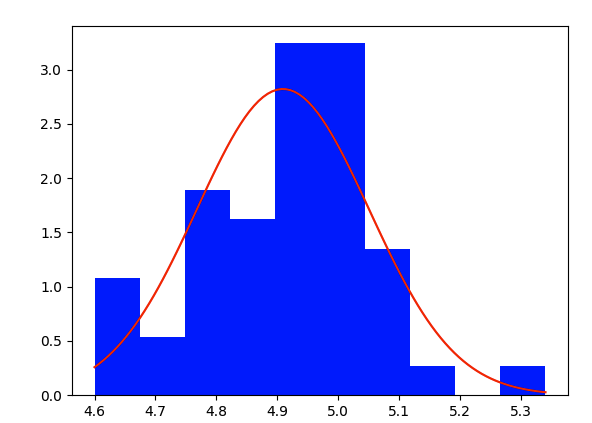
\includegraphics[scale=0.5]{grahp.png}}\\
	$\bar{x}=4.91$\\
	$SEM=0.143$\\
	$\sigma^2=0.141$\\
	$f_{max}=2.72$\\
	$\Delta{t}=[4.87, 4.95]$\\

\end{figure}



\section{Выводы}
Данные соответствуют ожидаемым результатам.\\Отклонения могут быть вызванны из-за нескольких факторов:
\begin{itemize}
	\item Недостаточность выборки, возможно если количество измерений было больше, то расхождений с теорией было бы меньше.
	\item В силу того, что человек смотрит на таймер, он пытается нажать чуть заранее, чтобы подать сигнал ровно в 5 секунд, отсюда и выходит что среднее значение чуть меньше 5 секунд.
	\item У каждого человека своя скорость реакции, которая к тому же может зависить от окружающих факторов и меняться с течением времени.
\end{itemize}
\end{document}
